\chapter{Инженерная реализация и эксплуатация предлагаемого решения}
\label{chap:Implementation}

\section{Требования к средствам обеспечения}
Основываясь на требованиях к аппаратному обеспечению, указанных в
Техническом задании (см. приложение
\ref{chap:RequirementsSpecification}), для инженерной реализации,
тестирования и эксплуатации системы автоматического извлечения
ключевых фраз из текста на естественном языке, характеристики
конфигурации \emph{сервера} не должны быть ниже следующих:
\begin{itemize}
  \item центральный процессор
Intel\textregistered~Core\textregistered~Duo или аналогичный по
производительности;
  \item оперативная память объёмом 2048 мегабайт;
  \item жёсткий диск объёмом 160 гигабайт;
  \item сетевая карта, работающая в полном дуплексе со
скоростью не менее 100 мегабит в секунду;
  \item операционная система: любая операционная система,
на которой возможен запуск виртуальной машины Rubinius
(например,
Red~Hat\textregistered~Enterprise~Linux\textregistered~Server~6
\cite{RHELS}).
\end{itemize}

Характеристики конфигурации \emph{рабочей станции пользователя}
для работы с системой не должны быть ниже следующих:
\begin{itemize}
  \item центральный процессор
Intel\textregistered~Pentium\textregistered~4 или аналогичный по
производительности;
  \item оперативная память объёмом 1024 мегабайт;
  \item жёсткий диск объёмом 160 гигабайт;
  \item сетевая карта, работающая в полном дуплексе со скоростью
не менее 10 мегабит в секунду;
  \item периферийные устройства:
  \begin{itemize}
    \item монитор;
    \item клавиатура;
    \item мышь.
  \end{itemize}
  \item операционная система: на выбор пользователя —
Microsoft\textregistered~Windows\textregistered,
GNU/Linux, Mac~OS~X, Oracle\textregistered~Solaris\texttrademark,
и\ др.
\end{itemize}

Инженерная реализация системы автоматического извлечения ключевых фраз
из текста на естественном языке выполнена на мультипарадигменном
языке программирования Ruby с использованием платформы Rubinius.

\section{Экранные формы}
Экранные формы разработанной системы автоматического извлечения
ключевых фраз из текста на естественном языке созданы в соответствии
со стандартом HTML5 \cite{HTML5}.

При обращении к системе, пользователю предлагается предоставить
исходный текст для обработки и выбрать формат, в котором будет
представлен результат работы системы: HTML, JSON или XML
(рисунок~\ref{fig:Implementation:Index}).

\begin{figure}[ht]
  \centering
  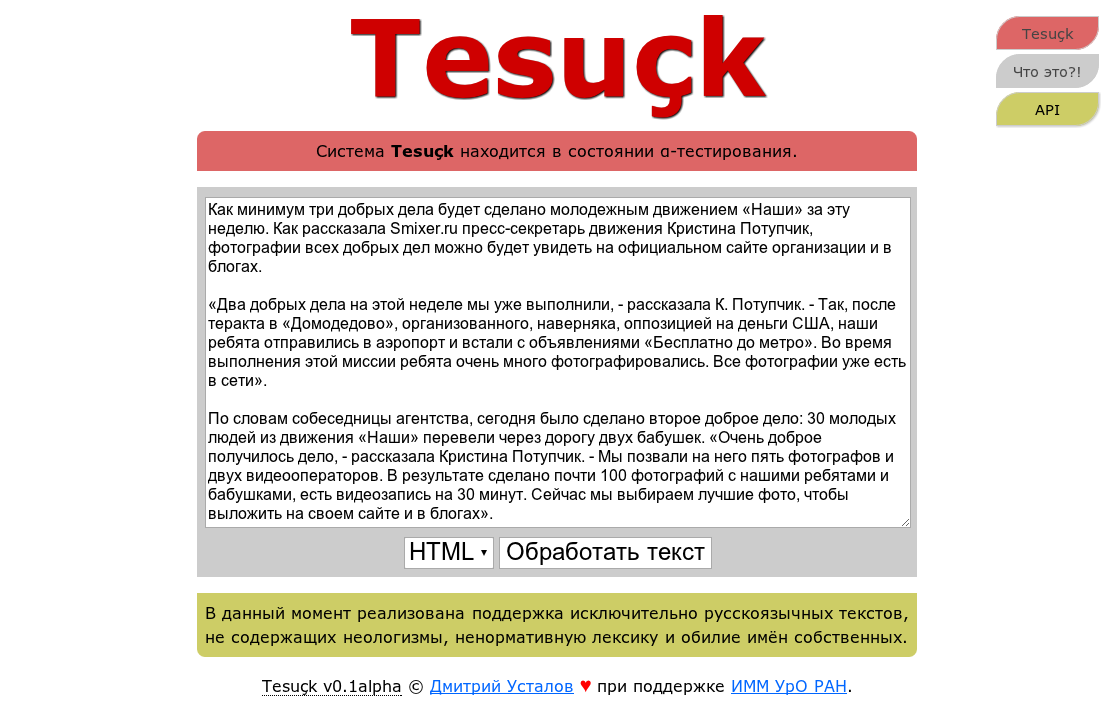
\includegraphics[width=\textwidth]{Tesuck-Index.png}
  \caption{Главная страница Web-интерфейса Tesuçk — системы
автоматического извлечения ключевых фраз из текста на
естественном языке}
  \label{fig:Implementation:Index}
\end{figure}

После выполнения запроса на обработку текста при выбранном формате
представления результатов HTML
(рисунок~\ref{fig:Implementation:Result}), система оформляет
результат в виде таблицы, состоящей из трёх колонок:
\begin{itemize}
  \item № — номер ключевой фразы, в соответствии с её значением
терминологичности;
  \item Ключевая фраза — именная группа, выделенная в качестве
ключевой фразы исходного текста;
  \item C-value — значение терминологичности, вычисленное в
соответствии с описанным в \ref{subsec:Solution}.
\end{itemize}

\begin{figure}[ht]
  \centering
  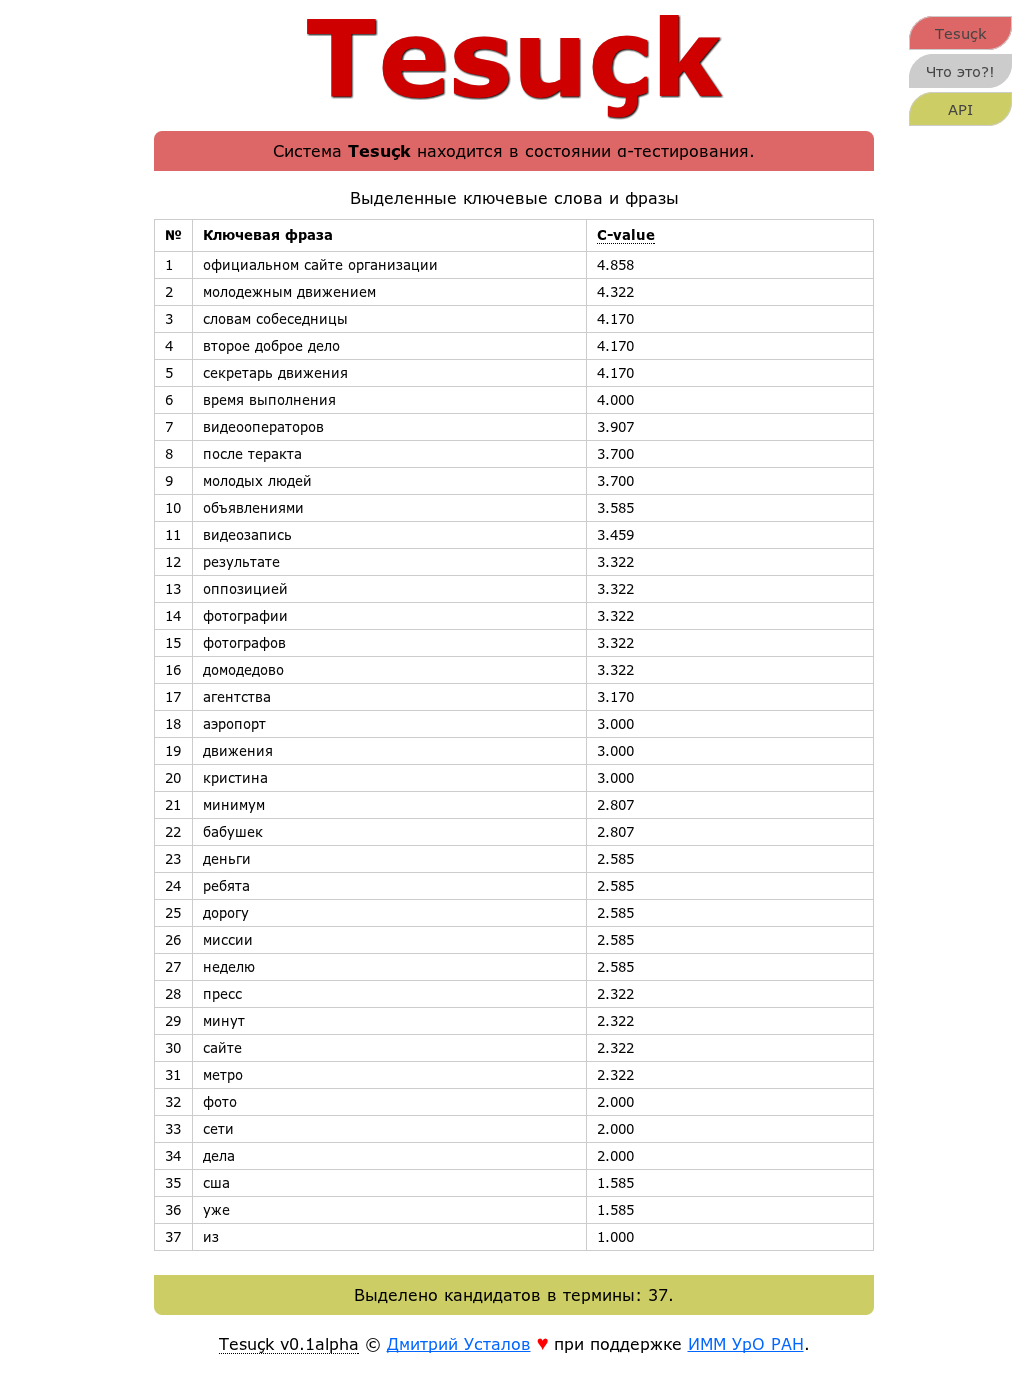
\includegraphics[width=\textwidth]{Tesuck-Result.png}
  \caption{Web-интерфейс представления результатов работы Tesuçk —
системы автоматического извлечения ключевых фраз из текста на
естественном языке}
  \label{fig:Implementation:Result}
\end{figure}

\section{Результаты и выводы}
В ходе инженерной реализации и эксплуатации разработанной системы
автоматического извлечения ключевых фраз из текста на
естественном языке, получены следующие результаты:
\begin{itemize}
  \item программно реализована система автоматического
извлечения ключевых фраз из текста на естественном языке;
  \item проведены эксперименты на работоспособность системы.
\end{itemize}
